\documentclass[t]{beamer}

\mode<handout>
{
  \usepackage{pgf}
  \usepackage{pgfpages}

\pgfpagesdeclarelayout{4 on 1 boxed}
{
  \edef\pgfpageoptionheight{\the\paperheight} 
  \edef\pgfpageoptionwidth{\the\paperwidth}
  \edef\pgfpageoptionborder{0pt}
}
{
  \pgfpagesphysicalpageoptions
  {%
    logical pages=4,%
    physical height=\pgfpageoptionheight,%
    physical width=\pgfpageoptionwidth%
  }
  \pgfpageslogicalpageoptions{1}
  {%
    border code=\pgfsetlinewidth{2pt}\pgfstroke,%
    border shrink=\pgfpageoptionborder,%
    resized width=.5\pgfphysicalwidth,%
    resized height=.5\pgfphysicalheight,%
    center=\pgfpoint{.25\pgfphysicalwidth}{.75\pgfphysicalheight}%
  }%
  \pgfpageslogicalpageoptions{2}
  {%
    border code=\pgfsetlinewidth{2pt}\pgfstroke,%
    border shrink=\pgfpageoptionborder,%
    resized width=.5\pgfphysicalwidth,%
    resized height=.5\pgfphysicalheight,%
    center=\pgfpoint{.75\pgfphysicalwidth}{.75\pgfphysicalheight}%
  }%
  \pgfpageslogicalpageoptions{3}
  {%
    border code=\pgfsetlinewidth{2pt}\pgfstroke,%
    border shrink=\pgfpageoptionborder,%
    resized width=.5\pgfphysicalwidth,%
    resized height=.5\pgfphysicalheight,%
    center=\pgfpoint{.25\pgfphysicalwidth}{.25\pgfphysicalheight}%
  }%
  \pgfpageslogicalpageoptions{4}
  {%
    border code=\pgfsetlinewidth{2pt}\pgfstroke,%
    border shrink=\pgfpageoptionborder,%
    resized width=.5\pgfphysicalwidth,%
    resized height=.5\pgfphysicalheight,%
    center=\pgfpoint{.75\pgfphysicalwidth}{.25\pgfphysicalheight}%
  }%
}


  \pgfpagesuselayout{4 on 1 boxed}[a4paper, border shrink=5mm, landscape]
  \nofiles
}

%% Language and font encodings
\usepackage[english]{babel}
\usepackage[utf8x]{inputenc}
\usepackage[T1]{fontenc}

\usetheme{Madrid}
\usecolortheme{beaver}

%% Useful packages
\usepackage{amsmath}
\usepackage{graphicx}

\usepackage{enumitem}

% full page itemieze
\newenvironment{fpi}
  {\itemize[nolistsep,itemsep=\fill]}
  {\vfill\enditemize}

\title{Transformations of Functions and \\
Exponential Functions}
\date{January 24, 2017}

\begin{document}
\frame{\titlepage}


\begin{frame}{Review of Section 1.2}
\begin{fpi}
\item Mathematical Models
\item Linear Regression
\item Function classes
\end{fpi}
\end{frame}

\begin{frame}{Review of Section 1.2}
Alice's parents recorded her height every 3 years when she was a child.
Find the linear regression.  Estimate her height at age 8.
\begin{tabular}{c c}
Age (years) & Heght
\hline
3 & 36 \\
6 & 42 \\
9  & 48 \\
12 & 60
\end{tabular}


\end{frame}

\begin{frame}{Review of Section 1.2}
\begin{fpi}
Classify the function as polynomial, power, rational, algebraic, trigonometric, exponential, or logarithmic.
\end{fpi}
\end{frame}

\begin{frame}{Review of Section 1.2}
\begin{fpi}
Classify the function as polynomial, power, rational, algebraic, trigonometric, exponential, or logarithmic.
\end{fpi}
\end{frame}

\begin{frame}{Outline of Section 1.3 (New Functions from Old)}
\begin{fpi}
\item Vertical and horizontal shifts
\item Vertical and horizontal stretching
\item Composition
\item Commonly seen classes of functions
\end{fpi}
\end{frame}

\begin{frame}{Mathematical models}
\vfill
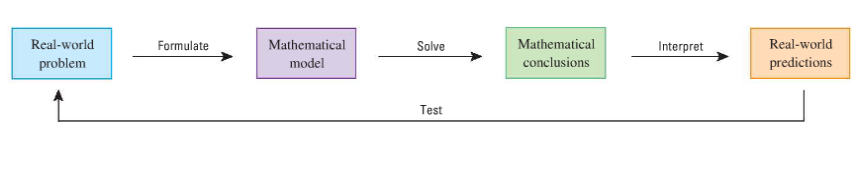
\includegraphics[width=\textwidth]{mmodel}
\vfill
\end{frame}


\begin{frame}{Linear functions}
\begin{itemize}
\item Linear refers to the fact that the graph forms a (straight) line
\vfill
\item Slope-intercept form:
$$y = mx + b$$
\vfill
\item Point-slope form:
$$y - y_0 = m(x - x_0)$$
\vfill
\end{itemize}
\end{frame}

\begin{frame}{Linear function example}
\begin{fpi}
\item $\displaystyle y = \frac{1}{2}x + 4$
\item $\displaystyle y - 1 = -2(x  +2)$
\end{fpi}
\end{frame}


\begin{frame}{Example}
Find the point-slope form of the line passing through the points
$(1,2)$ and $(0,3)$.
\end{frame}

\begin{frame}{Linear models}
\begin{fpi}
\item Given a table of $(x,y)$ data, we can approximate the data
with a linear function
\item This allows us to interpolate between the points and extrapolate beyond them
\item We can also make inferences about the whole data set
\end{fpi}
\end{frame}

\begin{frame}{Finding a linear regression using a TI-84}
\begin{fpi}
\item Press the STAT key.
\item Press Enter on the EDIT menu option
\item Fill the $x$ values into $L1$ and the $y$ values into $L2$.
\item Go to CALC menu option and select LinReg($ax + b$).
\item This gives you the equation of the line.
\item Press Y= to see the graph.
\end{fpi}
\end{frame}

\begin{frame}{Finding a linear regression using Wolfram Alpha}
Type in ``Linear Regression'' and then list your $(x,y)$ pairs, e.g.
$$\text{Linear Regression } [[1,2], [2,2],[3,4]]$$
\end{frame}


\begin{frame}{Linear model example}
The Dallas News reported these attendance
numbers from 2014:
\begin{fpi}
\item Baylor – 46,710
\item North Texas – 19,271
\item  Oklahoma – 85,162
\item  SMU – 21,528
\item  TCU – 44,719
\item  Texas – 94,103
\item  Texas A\&M –105,123
\item  Texas Tech – 58,934
\end{fpi}
\end{frame}

\begin{frame}{Linear model example}
\vfill
 How much does the size of the school affect football attendence?  
\vfill
\end{frame}

\begin{frame}{Linear model example}
\vfill
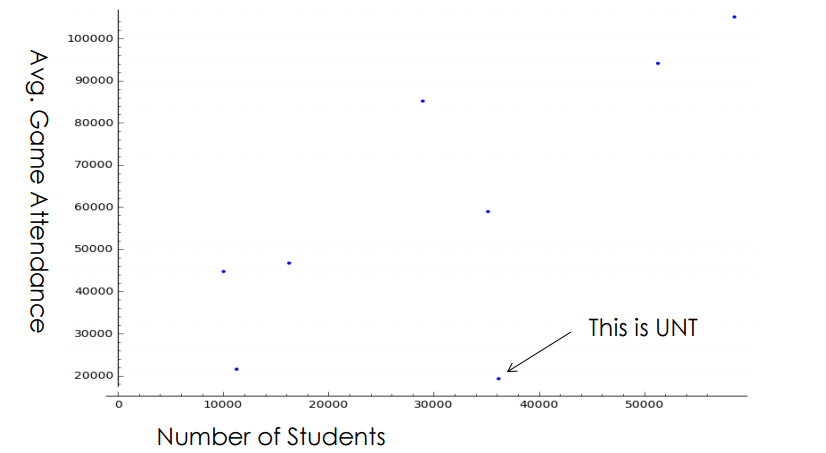
\includegraphics[width=\textwidth]{football}
\vfill
\end{frame}

\begin{frame}{Linear model example}
The linear regression line is
$$y = 1.3x + 19202$$
\end{frame}


\begin{frame}{Linear model example}
\vfill
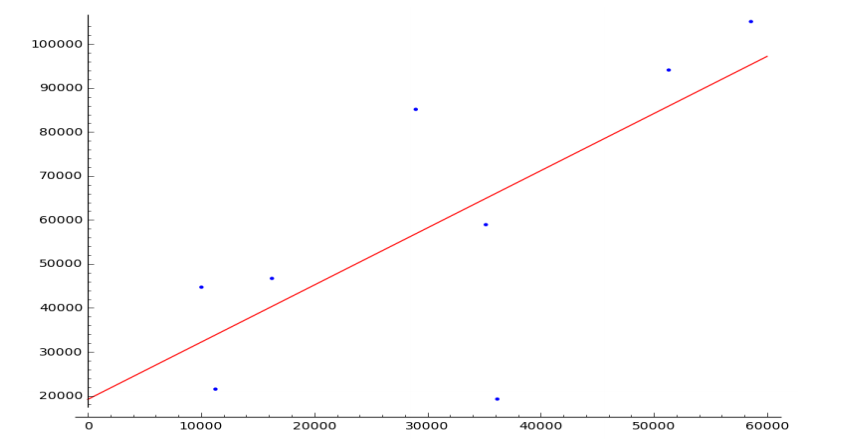
\includegraphics[width=\textwidth]{football2}
\vfill
\end{frame}

\begin{frame}{Football example: Interpolation}
If a new university in Texas had a student population of
$10000$, what would be the expected football attendance?
\end{frame}

\begin{frame}{Polynomials}
\begin{fpi}
\item A \textbf{polynomial} is a function that looks like
$$y = 2x^5 + 3x^3 -2x^2 + 3x + 1$$
\item The general form of a polynomial is
$$y = a_n x^n + a_{n-1} x^{n-1} + \cdots + a_1 x + a_0$$
where the \textbf{coefficients} $a_i$ are just numbers.  
\item The highest 
exponent of $x$ appearing in the polynomial is called its \textbf{degree}.
\end{fpi}
\end{frame}

\begin{frame}{Quadratic polynomials}
\begin{block}{Definition}
A \textbf{quadratic polynomial} is a polynomial of degree 2.
\end{block}
\begin{block}{Example}
$$f(x) = 3x^2 - 2x + 1$$
\end{block}
\begin{block}{General form}
$$f(x) = ax^2 + bx + c$$
\end{block}
\end{frame}

\begin{frame}{Graphs of quadratic functions}
\vfill
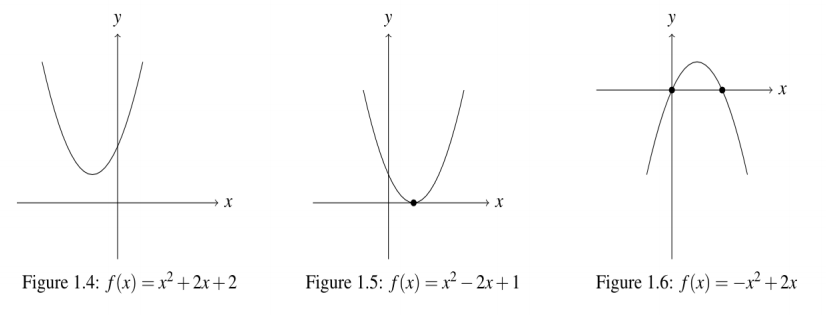
\includegraphics[width=\textwidth]{quadratic}
\vfill
\end{frame}

\begin{frame}{Graphs of more general polynomials}
\vfill
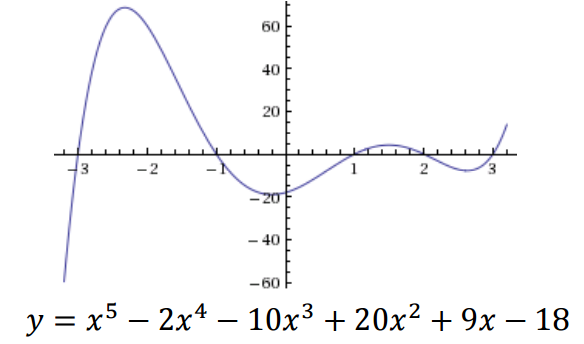
\includegraphics[width=\textwidth]{poly}
\vfill
\end{frame}

\begin{frame}{Power functions}
\begin{block}{Definition}
A \textbf{power function} is a function of the form
$$y = x^a,$$
where $a$ is a constant.
\end{block}
Three cases:
\begin{itemize}
\item $a$ is a positive integer.
\item $a$ is a fraction
\item $a$ is a negative number.
\end{itemize}
\end{frame}

\begin{frame}{Power functions with positive integer exponents}
\vfill
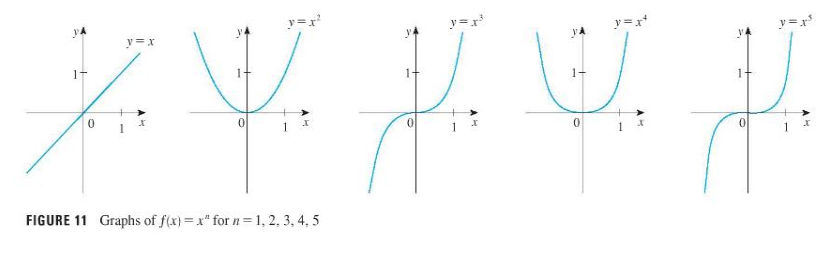
\includegraphics[width=\textwidth]{posint}
\vfill
\end{frame}

\begin{frame}{Power functions with fractional exponents}
\vfill
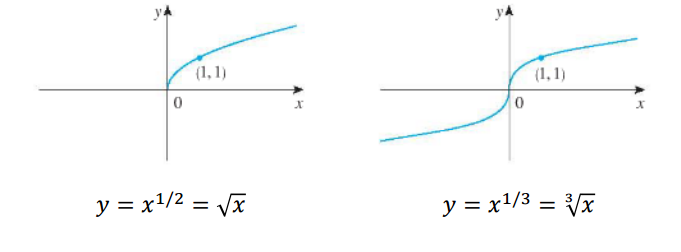
\includegraphics[width=\textwidth]{fraction}
\vfill
\end{frame}

\begin{frame}{Power functions with negative exponents}
\vfill
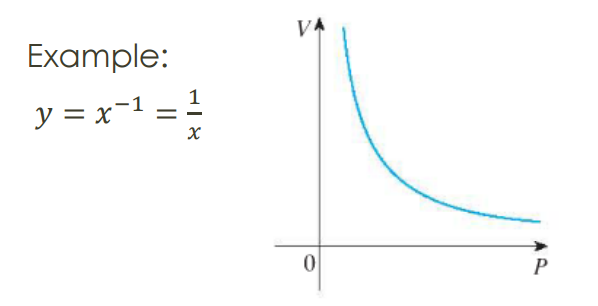
\includegraphics[width=\textwidth]{negative}
\vfill
\end{frame}

\begin{frame}{Rational functions}
\begin{block}{Definition}
A \textbf{rational function} is a ratio of two polynomials.
\end{block}
\begin{block}{Example}
$$f(x) = \frac{3x^2 - x+ 3}{2x+1}$$
\end{block}
\begin{block}{General form}
$$f(x) = \frac{P(x)}{Q(x)},$$
where $P(x)$ and $Q(x)$ are polynomials.
\end{block}
\end{frame}

\begin{frame}{Rational functions}
\vfill
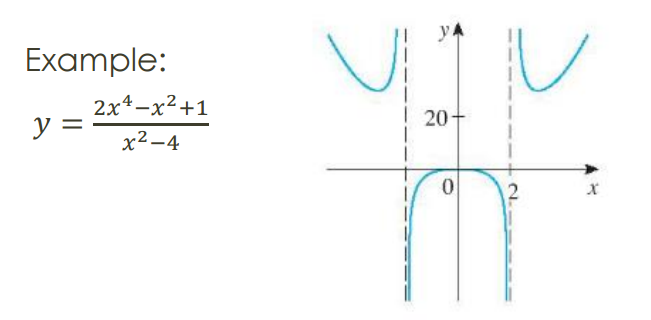
\includegraphics[width=\textwidth]{rational}
\vfill
\end{frame}

\begin{frame}{Algebraic functions}
An \textbf{algebraic function} is like rational function, but we also
allow taking roots.
\begin{block}{Example}
$$f(x) = \frac{\sqrt{3x^2 - x}}{3x+1} + x\sqrt[3]{x-1}$$
\end{block}
\end{frame}

\begin{frame}{Algebraic functions}
\begin{figure}
\vfill
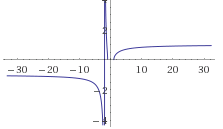
\includegraphics[width=0.5\textwidth]{algebraic}
\caption{$\displaystyle y = \frac{\sqrt{x^2 -1}}{x + 2}$}
\end{figure}
\vfill
\end{frame}

\begin{frame}{Trig functions}
\begin{fpi}
\item The trig functions are $\sin(x)$, $ \cos(x)$ and their ratios and inverses.
\item All of them are $2\pi$-periodic
\item For all $x$,
$$-1 \le sin(x) \le 1 \qquad \text{ and }\qquad -1 \le \cos(x) \le 1$$
\end{fpi}
\end{frame}


\begin{frame}{Exponential functions}
\begin{block}{Definition}
An exponential function is a function of the form
$$ f(x) = a^x,$$
where $a$ is a positive number.
\end{block}
\end{frame}

\begin{frame}{Logarithmic functions}
\begin{block}{Definition}
A logarithmic function is a function of the form
$$ f(x) = \log_a x,$$
where $a$ is positive constant.
\end{block}
\end{frame}


\end{document}
